\chapter{绪论}

\section{研究背景及意义}

近年来,喷水推进泵在高速船舶推进系统中得到了广泛应用,
随着动力传动系统与船体减振降噪技术的进步,推进泵噪声对舰船总体噪声的贡献度也被相对提高,
因而目前高新船舶对高效低噪声推进泵的需求日益迫切。
在满足推进性能需求的基础上,振动与声学特性目前已成为推进泵优化设计所关注的重点。
无论从推进泵低噪声设计或是从水声信号识别角度,对推进泵噪声的特性与机理开展研究均具有重要意义。
推进泵噪声机理较为复杂,抛开空化噪声不谈仅从流致噪声角度考虑,其频谱已呈现宽带与线谱交叠的形貌,
其中线谱噪声对噪声总级贡献度较大,很大程度上决定了推进泵的噪声水平。
前期研究发现,推进泵叶轮与其他部件之间的动静干涉是重要的线谱噪声激励源,
动静干涉的抑制因此成为降低推进泵线谱振动与噪声的有效方法之一。

(1)从调制与解调的基本概念出发,采用基于循环平稳信号分析手段对推进泵噪声信号进行解调研究,
重点分析了推进泵的噪声调制特征机理,得到了在进速系数下的解调谱。
(2)基于labVIEW平台开发了推进泵振动噪声测试系统,开展了振动及噪声信号频率和特征、信号特征频段等研究,
为进行推进泵振动噪声测量、判断推进泵声学性能及进行噪声及流致激励源特性分析奠定了研究基础。 


\section{研究现状}
\subsection{推进泵噪声及流致激励源研究现状}
目前,国内外已经围绕螺旋桨、对转桨、推进泵等多种类型推进器的噪声开展了研究,
在噪声理论模型与噪声调制机理方面已有较多研究成果。
史广智[5]等人基于螺旋桨节拍对螺旋桨空化噪声的调幅作用,
研究了螺旋桨空化噪声理论模型与谐波族的关键特征。
曾赛[6]等人基于声学类比法建立了对转桨无空化噪声调制模型,研究了对转桨噪声的调制机理。
苏永生[7]等人分析了单级喷水推进泵空化噪声的调制特征,并研究了空化程度与噪声的关系。
总的来说,推进器伴流场谐调频率、叶片数与线谱噪声之间存在密切联系,
而循环平稳分析方法则是解调、量化这种联系的有效手段。

\subsection{循环平稳信号分析手段}
推进器、泵等旋转机械的噪声信号是周期性时变的,具有典型的循环平稳特征[8]。
其噪声信号常用的解调方法含包络分析、循环平稳分析等非平稳信号分析方法。
从解调调幅信号角度来看,在频率域上的包络谱分析方法等效于在循环频率域上的循环平稳分析方法,
但包络谱分析完全忽略了载波信息,无法揭示载波频率[9-10]。
而循环平稳自相关分析方法不仅具备包络谱分析的解调效果,可提取出调制特征信号,
同时具备功率谱密度分析方法的功效,可更好地支撑旋转机械噪声机理分析。
近年来,循环平稳分析方法开始用于机械故障检测以及旋转机械信号特征提取领域。
Antoni[11]较早研究了循环平稳分析方法在旋转机械噪声分析中的应用。
李诗佯[12]等人将CFD(计算流体力学)方法和循环平稳分析方法相结合,
建立了离心泵振动信号的幅值调制模型,研究了离心泵流致振动机理。
总的来说,对于信噪比低的旋转机械信号,例如处于复杂水声环境中的船舶推进器噪声,
循环平稳分析比包络谱分析具有更好的解调能力。

\section{研究内容和目标}
\subsection{研究内容}
\subsection{研究目标}

\chapter{推进泵振动噪声测试系统设计}
\section{引言}
本文基于LabVIEW平台开发了推进泵振动噪声测试系统,其中涵盖了信号采集的硬件系统设计,
以及实现信号分析和存储的软件系统设计,该系统支持同步对多通道传感器信号实时采集,各通道信号同时处理、显示及存储,
同时也能够实现振动加速度传感器的性能检验和指标评估,适用于各类泵和风机振动及噪声测试场景。

基于此平台可开展对振动及噪声信号频率和特性、特征频段等研究,
为进行推进泵振动噪声测量、判断推进泵声学性能及进行噪声及流致激励源特性分析奠定了研究基础。

\section{系统总体设计概述}
\subsection{测试基本参数和数据处理}
本文设计的测试信号对象包括声压和振动加速度信号,用来表征测试对象的声学和振动性能,可分别由麦克风或者水听器和
振动加速度传感器测量。信号处理主要涉及频谱分析和1/3倍频程分析。

在振动与噪声信号的分析中,声压级和振动加速度级是常用的参数,一个声学量的级是该量与同类量的基准值之比的对数。
其中,声压级定义为将待测声压$p_e$与参考声压$p_{ref}$的比值取常用对数,再乘以20,以分贝计,即
\begin{equation}
    \label{equ:p}
    L_{p} = 20\log_{10}{\left(p_{re}/p_{ref}\right )}
\end{equation}
式中,在水中基准声压为$p_{ref}= 1\times 10^{-6} \mathrm{P} a$,在空气中基准声压为$p_{ref}= 2\times 10^{-5} \mathrm{P} a$。
同理,振动加速度级也定义为加速度有效值$a_e$与基准加速度$a_{ref}$之比的以10为底的对数,再乘以20,以分贝计,即
\begin{equation}
    \label{equ:a}
    L_{a} = 20\log_{10}{\left(a_{re}/a_{ref}\right )}
\end{equation}
式中,基准加速度值为$a_{ref}= 1\times 10^{-6} \mathrm{m/s^2} $。

信号的频谱是指信号的频率成分与能量分布的关系,可以体现信号的频率特征。在振动与噪声信号的分析中,
通常也会采用1/3倍频程频谱分析,是比较符合人耳分辨频率能力的频带划分方法,能更加详细的反映噪声源的频谱特性。
通过将整个频谱划分为若干频带,每个频带的上限频率$f_u$与下限频率$f_l$之比是2的立方根,即满足以下公式:
\begin{equation}
    \label{equ:fu}
    f_{u}/f_{l}=2^{1/3}=1.2599
\end{equation}
中心频率f$_{m}$为上下限频率的几何平均值,即
\begin{equation}
    \label{equ:fm}
    f_{m}=\sqrt{f_{u}\cdot f_{l} } 
\end{equation}
本文进行1/3倍频程分析所采用的方法是通过对采样信号进行快速傅立叶变换,计算出功率谱或幅值谱,
然后用功率谱或幅值谱的数据,计算每一个中心频率带宽的信号有效值,代入\autoref{equ:p}或\autoref{equ:a}
中可得到该频段内的声压级。
\subsection{测试系统基本方案}
本文所采用的技术框架如\autoref{fig:framework}所示,主要包括传感器,信号调理模块,数据采集卡和上位机分析软件。
\begin{figure}[htbp]
    \centering
    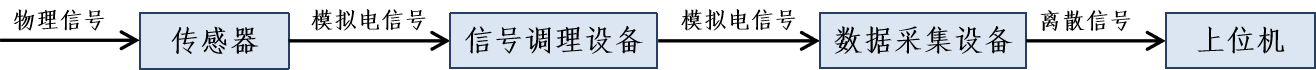
\includegraphics[scale=0.55]{2硬件设备流程图.png}
    \caption{\label{fig:framework}技术框架图}
\end{figure}

目前国内在数据采集卡和上位机分析软件的结合方面主要采用的方式有两种,
一种是购买国内公司的数据采集卡,然后自行设计上位机分析软件,这种方案价格低廉,
但是自行开发上位机软件周期长,且功能有限还不易扩展。
另一种是购买美国NI公司的LabVIEW软件和数据采集卡套件,NI公司的虚拟仪器系统灵活性高,
开发成本更低,同时数据采集卡套件系统具有更小尺寸,但是价格非常高昂。
针对本文所涉及的泵或风机等测试场景,选用开发灵活性更高且尺寸更小的硬件系统更为合适,
因此本文采用的是美国NI公司的LabVIEW软件和数据采集卡套件。

LabVIEW通过调用硬件设备的底层驱动程序,结合软件功能模块,从而搭建出控制数据采集传输,处理和存储的系统。
该系统的的核心部分是功能模块的设计,本系统功能模块可分为系统设置模块、信号采集模块、数据显示模块、信号分析模块、数据管理模块等,
系统方案图如\autoref{fig:system}所示。此外还可以根据实际情况,灵活地添加新的功能模块。
在2.3节软件系统设计中将对软件模块的设计过程作详细介绍。
\begin{figure}[htbp]
    \centering
    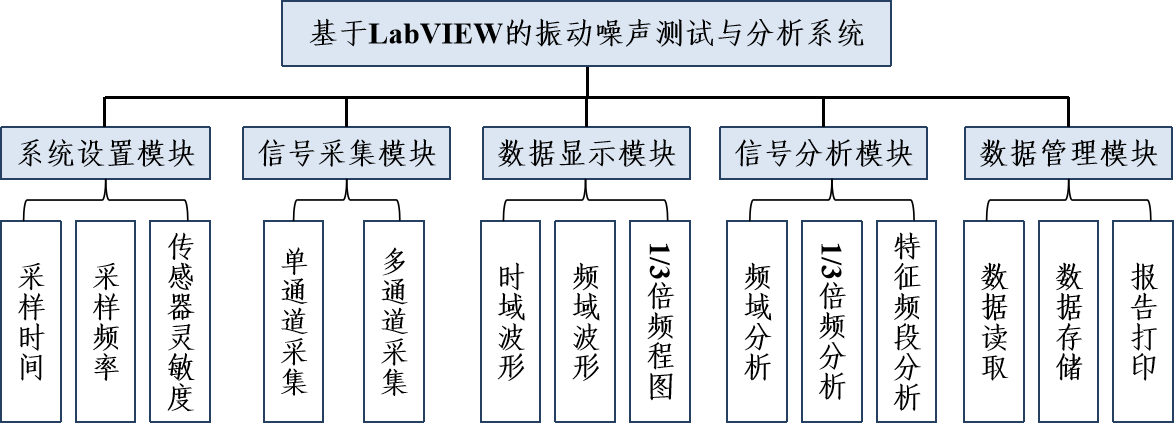
\includegraphics[scale=0.6]{2系统方案.png}
    \caption{\label{fig:system}系统方案图}
\end{figure}

\section{硬件系统设计}
针对本文所涉及的泵或风机等测试场景,传感器需要支持远距离传输,简单电路调理等功能,
因此本文选用了抗干扰能力强,内置放大器等要求的传感器类型。
传感器由于内置了专门的集成调理电路,属于有源传感器,而该电路要正常工作需要恒流源供电。
这样一来,一方面系统可以不用设置额外的信号调理设备,简化了测试系统。
另一方面对数据采集设备也提出了要求,主要包括以下几个方面,(1)支持多通道同步采集;
(2)支持IEPE信号调理;(3)轻巧灵活,便携式;(4)支持USB外设总线技术。

综合考虑以上因素,本文选用了​NI9234采集卡,如\autoref{fig:acquire}所示。
​NI9234是美国NI公司的一种4通道高速动态信号采集卡,兼容USB接口,AC/DC耦合方式可选,
可对IEPE传感器进行高精度测量。
NI9234带有2mA恒定电流的集成电路压电式(IEPE)信号调理,包含内置抗混叠滤波器,
可自动调节至设置的采样率,也对采集系统进行了接地屏蔽处理,
输入通道可同时以最高为51.2$\mathrm{kHz}$的速率对信号进行数字化。
\begin{figure}[htbp]
    \centering
    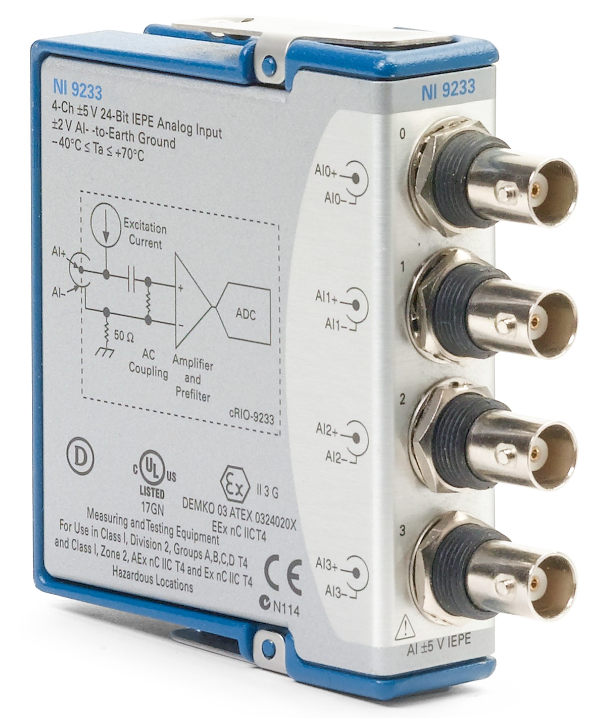
\includegraphics[scale=0.3]{2数据采集卡.png}
    \caption{\label{fig:acquire}数据采集卡}
\end{figure}
​
数据采集卡每个通道的输入信号经缓冲,放大器和预滤波器调理后,由模数转换器对其采样。

数据采集卡系统结构如\autoref{fig:acquire}所示。
数据采集卡采集数据时,数据传输方式包括直接内存访问(DMA),中断请求(IRQ)和可编程I/O。
DMA是一种DAQ板卡和PC内存间直接通讯的传输方式,不再需要处理器的干预。
NI "MITE"芯片可以处理与PCI总线间的所有总线协议。
IRQ传输方式会置高信号并中断处理器,然后由处理器处理数据传输。
IRQ  传输通常很低,只有150 kb/s,而DMA可以高达20 Mb/s。
IRQ 传输速率与使用的系统设备相关,如处理器速度等。
NI数据采集系统中默认是使用DMA传输方式。

数据采集卡的传输过程为,外部的信号进入数据采集卡后,经过各种处理转换,
先进入数据采集卡自身的缓冲区里面,缓冲区是先进先出(FIFO,First In First Out)的。
NI的数据采集卡有板载的缓冲区,不同数据采集卡的缓冲区的大小不一样,
板载缓冲区的大小一般是出厂商固定的,无法更改。
然后当板载缓冲区中的数据量到了一定的条件时,数据采集卡将缓冲区的数据上传到计算机内存中,
一般是以DMA(直接内存访问)方式传入的。

\begin{figure}[htbp]
    \centering
    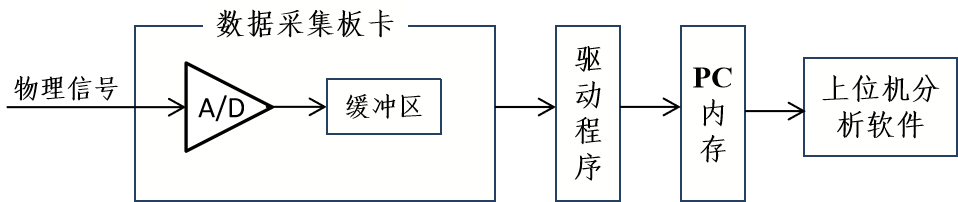
\includegraphics[scale=0.6]{2数据采集卡系统结构.png}
    \caption{\label{fig:acquire}数据采集卡系统结构}
\end{figure}

\section{软件系统设计}
在对软件系统进行设计之前,最先需要考虑的是计算机与硬件的交互。
和硬件交互需要两个基本要素:第一,硬件和计算机的通信接口和通信协议。
常用的接口及协议有RS232 、GPIB、USB 、LAN,以及VXI 和PXI通信总线等等;
第二,交互命令,即通过上述通信接口按照协议发送的逻辑程控指令,例如仪器程控中常见的有VISA 、SCPI命令架构体系。

LabVIEW最大优势就是和测量硬件交互的便利性。
因为一方面NI公司将与硬件交互的逻辑指令按功能组织成硬件驱动(driver),可以直接下载安装。
另一方面NI的数据采集板卡一般都支持多种外设总线技术,比如ISA、PCI、 Firewire、USB 和PCMCIA,
外设总线的作用是允许外部IO设备与计算机CPU和内存通信。
使用LabVIEW连接硬件系统往往需要一个工具软件NI的MAX,即Measurement\&Automation Explorer(MAX),
用来验证驱动安装与否和连接的正常性检查。
在我们安装好驱动之后,用NI MAX软件验证连接和驱动的工作正常性,
之后就可以开始在LabVIEW中进行编程来实现具体的业务功能。

LabVIEW是图形化的编程语言,编程方法不同于传统程序设计方法, 它摆脱了传统语言线性结构的困扰, 
执行顺序是由数据流的方式确定。
本文基于LabVIEW面向过程的编程思想,使用了通知器、队列和事件的设计模式,
实现了系统设置模块、信号采集模块、数据显示模块、信号分析模块、数据管理模块等模块的设计。
软件的主界面如\autoref{fig:main}所示,各功能模块集成到该主界面上。
\begin{figure}[htbp]
    \centering
    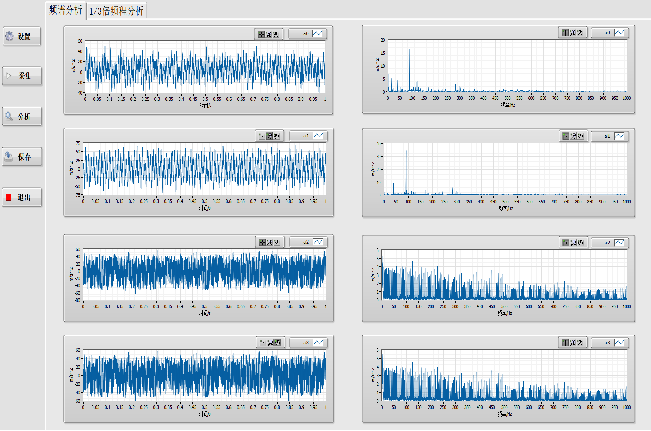
\includegraphics[scale=0.25]{2软件主界面.png}
    \caption{\label{fig:main}软件主界面}
\end{figure}

推进泵振动或噪声测试系统测量流程是:首先等待各部分参数设置好后,发出采集启动信号,
同步采集各通道数据,采集完成后数据自动存储在相应文件中。信号分析会从文件中读取数据,
分析结果实时展示在界面。程序设计流程如\autoref{fig:process}所示。
\begin{figure}[htbp]
    \centering
    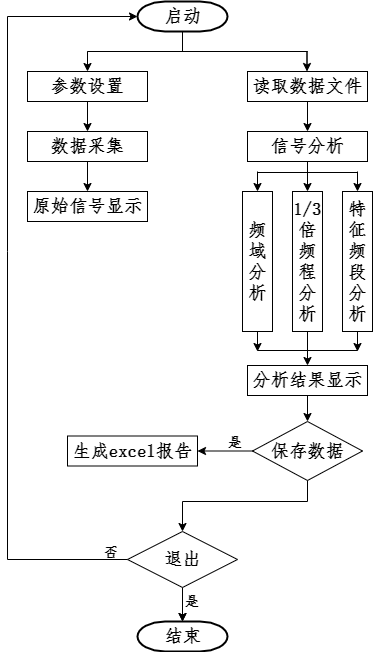
\includegraphics[scale=0.55]{2软件流程图.png}
    \caption{\label{fig:process}程序流程图}
\end{figure}

\subsection{系统设置模块}
软件界面的设置模块提供了测试系统各项参数设定,包括采集通道设置、采样参数设置、
传感器灵敏度设置、分析参数设置等。
\begin{figure}[htbp]
    \centering
    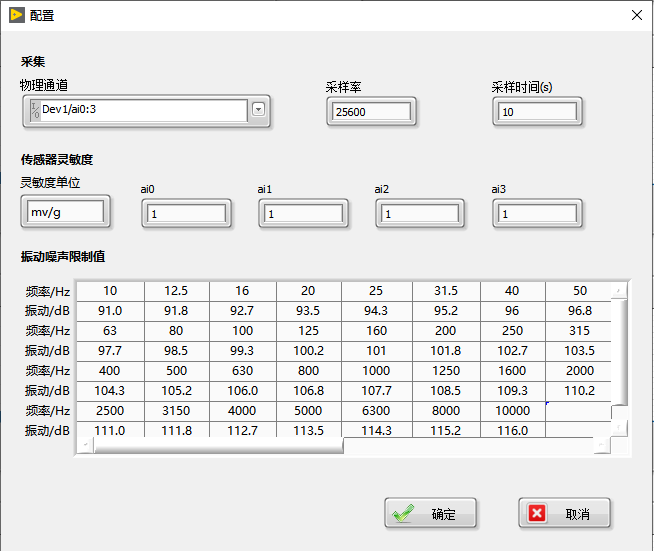
\includegraphics[scale=0.55]{2系统设置.png}
    \caption{\label{fig:setting}系统设置}
\end{figure}

\subsection{数据采集模块}
在对数据采集模块进行设计时,本文主要考虑如下几个方面:(1)如何保证数据在采集过程中不丢失?
(2)实现采集数据的实时存储。
在2.2节提到程序最终是从计算机内存读取数据,而这个缓存区的大小是我们可以指定的。
缓冲区存储数据量的大小又是和它的输入速度和输出速度有关,输入速率是由采样率所决定的,
输出速度就是采集程序从它里面读取的速度。
假如计算机内存缓冲区设置的过小,或者输出速率过慢,都有可能导致缓存区的溢出,出现数据丢失的情况。
计算机内存缓冲区设置的过大,在硬盘和内存之间会产生过量的读写操作,也会对系统性能造成影响。
所以为了保证数据不会丢失,要设置好内存缓冲区的大小,
还要保证读取缓冲区的程序(DAQmx Read.vi)循环得尽量快,每一次读取的数据尽量多。
LabVIEW中缓冲区大小的设置也和采样模式有关,常用的采样模式为有限采样和连续采样,本文采用连续采样模式。
对于连续采样模式,NI-DAQmx设置的缓存区大小如\autoref{tab:sample}所示,缓存区大小建议是采样率的10倍左右。
对于读取缓冲区的程序(DAQmx Read.vi)来说,设置成多采样,每次都是将内存中的所有数据读取进来,就能实现读取的数据尽量多。
\begin{table}[htbp]
    \centering
    \caption{\label{tab:sample}NI-DAQmx连续采样缓存区大小}
    \begin{tabular}{ccc}
     \toprule
     采样率&缓冲区大小\\
     \midrule
     未指定速率&10 kS\\
     0-100 S/s&1 kS\\
     100-10,000 S/s&10 kS\\
     10,000-1,000,000 S/s&100 kS\\
     >1,000,000 S/s&1 MS\\
     \bottomrule
    \end{tabular}
\end{table}

为实现数据的实时存储,本文采用了生产者/消费者的模式,
生产者/消费者结构基于队列的数据结构,即开辟一个缓存区,依据先进先出的原则进行。
新来的元素总是被加入队尾,每次离开的元素总是从队首离开。程序中新采集的数据加入到
队尾,队首出队的元素同步保存在相应文件中。
这样就保证了数据存储过程中不会出现数据丢失的现象,能实现实时存储。
数据采集程序框图如\autoref{fig:soft}所示。
\begin{figure}[htbp]
    \centering
    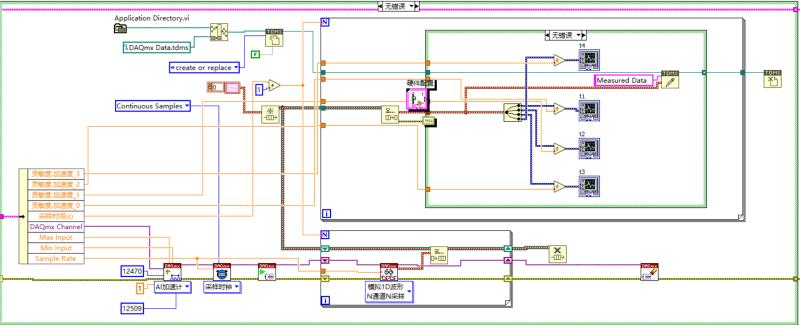
\includegraphics[scale=0.85]{2数据采集程序框图.jpg}
    \caption{\label{fig:soft}数据采集程序框图}
\end{figure}


\subsection{信号分析模块}
LabVIEW以G编程语言为基础,尤其适合于数据采集、仪器控制、和图像显示等应用,可以高效地构建虚拟仪器系统。
然而这种图形化的软件开发环境对于复杂的数值计算和分析要求就显得力不从心,
在对各种信号分析算法的支持方面,LabVIEW的工具箱也非常有限。
LabVIEW8.2以后版本推出了仿真框图和面向数学的文本编辑语言MathScript,它带
有交互式窗口和可编辑的接口,通过MathScript用户可以在LabVIEW图形化程序中运行较简单的m文件语法脚本。
因此LabVIEW提供了与MATLAB进行通信的方式,本文借助数据处理能力更强的MATLAB进行信号的分析。

MATLAB也支持ActiveX自动化技术,LabVIEW程序在运行MATLAB Script节点时,会启动一个MATLAB进程执行脚本的内容,
并且与MATLAB的工作空间进行数据交换。但是MATLAB Script节点对输入、输出数据的类型有明确的要求,只有
LabVIEW中的数据类型与MATLAB中的数据类型相匹配,才能够进行数据交换。
将采集模块中获取的数据导入如\autoref{fig:otc}所示的节点中,便可对信号进行频谱分析和1/3倍频程分析,
软件分析模块的界面如\autoref{fig:analyze}所示。
\begin{figure}[htbp]
    \centering
    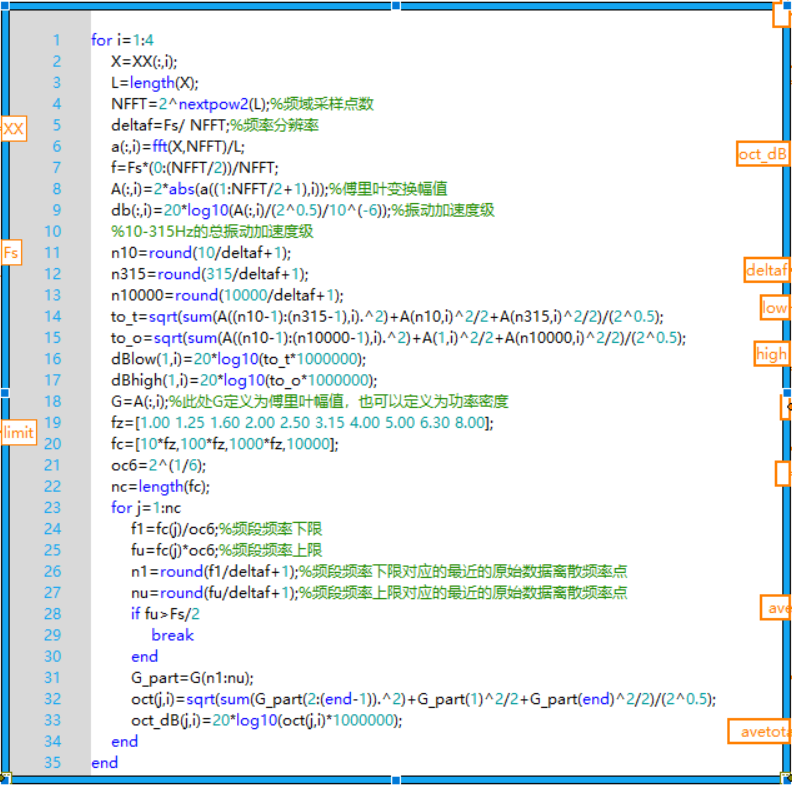
\includegraphics[scale=0.75]{2倍频程程序.png}
    \caption{\label{fig:otc}mathscript节点部分进行1/3倍频程分析的程序}
\end{figure}

\begin{figure}[htbp]
    \centering
    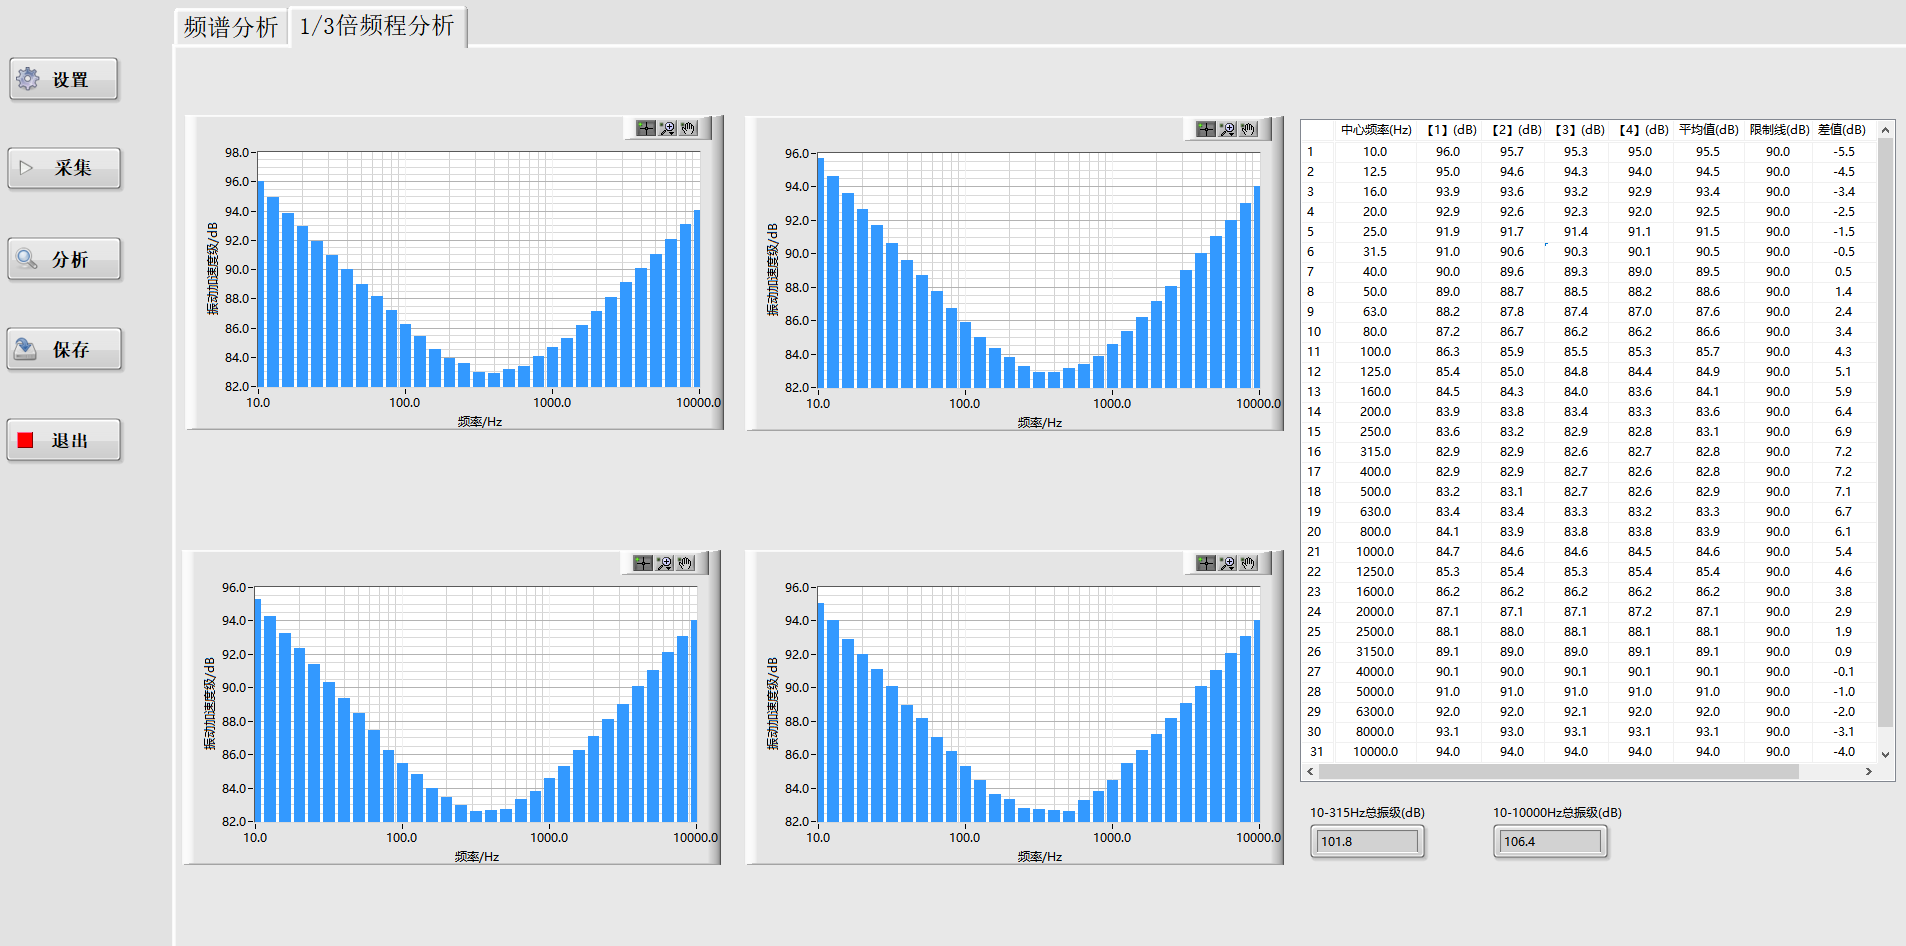
\includegraphics[scale=0.25]{2软件分析模块.png}
    \caption{\label{fig:analyze}mathscript节点部分进行1/3倍频程分析的程序}
\end{figure}

\subsection{数据管理模块}
数据管理模块包含采集数据的实时存储、采集数据的读取和分析数据的存储。
由于实验是多通道数据采集,且采样速度要求较高,因此数据量较大。为了方便实时存储和
管理这些数据,程序采用TDMS文件格式。TDMS文件格式是NI主推的一种二进制记录文件,
它兼顾了高速、易存取和方便等多种优势,在记录的仿真或测量数据的同时,也会存储描述性信息,
包括测试过程,传感器信息等,数据实时存储程序框图如\autoref{fig:save}所示。当数据采集完成进行分析时,程序会从已保存的TDMS文件中读取数据
导入分析模块进行,数据读取程序框图如\autoref{fig:read}所示。分析完成数据将会以excel表格的形式进行存储。
主程序中从VISAread的readbuffer端读上来的数据需要转换成表格数据进行保存,
数据的保存分为两个阶段。第一阶段,通过表单形式(带时间头)显示在主程序界面,
方便用户直观查看测试参数是否已满足要求。
第二阶段,把表单数据保存到Excel文件中,可供用户打印查询。
\begin{figure}[htbp]
    \centering
    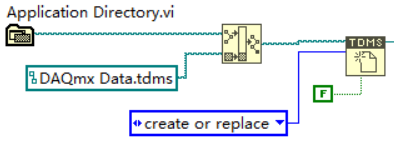
\includegraphics[scale=0.85]{2文件存储.png}
    \caption{\label{fig:save}数据实时存储程序框图}
\end{figure}
\begin{figure}[htbp]
    \centering
    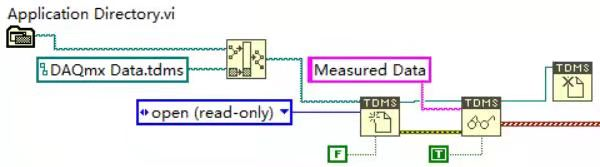
\includegraphics[scale=0.45]{2文件读取.jpg}
    \caption{\label{fig:read}数据读取程序框图}
\end{figure}
\section{性能测试}
\section{本章小结}
本章针对推进泵噪声试验平台振动噪声测试系统中的硬件系统设计和软件系统设计,
采用美国pcb手持式校准器394C06进行校准。

\chapter{推进泵噪声特性的试验研究}
\section{引言}
\section{推进泵试验台简介}
本文依托上海船舶运输研究所(SSSRI)的空泡水洞,针对推进泵样机模型开展了水动力性能和噪声性能的试验研究。
空泡水洞由德国KEMPF\&REMMERS公司制造,如\autoref{fig:tube1}和\autoref{fig:tube2}所示。
\begin{figure}[htbp]
    \centering
    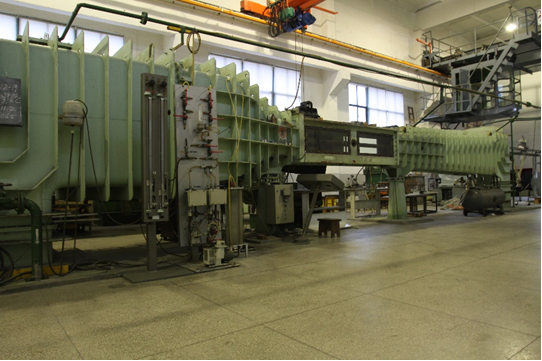
\includegraphics[scale=0.85]{3水洞1.png}
    \caption{\label{fig:tube1}SSSRI空泡水洞}
\end{figure}
\begin{figure}[htbp]
    \centering
    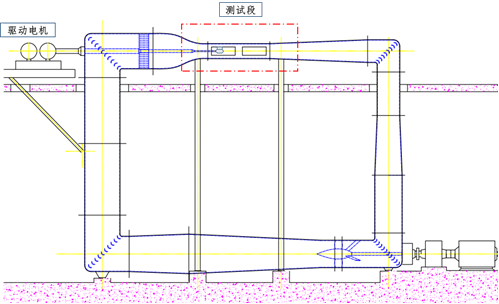
\includegraphics[scale=0.85]{3水洞2.png}
    \caption{\label{fig:tube2}水洞整体结构}
\end{figure}
水洞整体采用不锈钢材料,配有压力调节箱和除气装置,具有很好的可控性。
水洞工作段长2.6m,横截面呈方形带圆角,尺寸为0.6m×0.6m。
水洞工作段的压力调节范围为10~200kpa,最高水速可达12m/s,最低水速空泡数为0.2。
缩比模型样机悬挂于水洞上壁面,导管由光折射率与水一致的透明有机玻璃制成,以确保其内流场的可视性。
水筒侧面有机玻璃外安装一小型水舱,将水听器阵列置于其中,测量推进泵在多工况下运转的水下噪声。


推进泵噪声测试系统的示意图如\autoref{fig:equipment}所示,主要包括测试推进泵、水洞、水听器、
数据采集卡、电脑(上位机软件)五部分组成。
\begin{figure}[htbp]
    \centering
    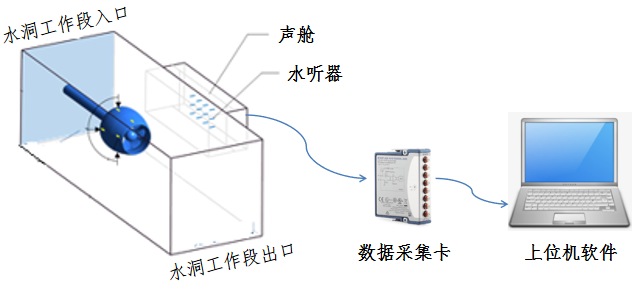
\includegraphics[scale=0.85]{3测试系统.png}
    \caption{\label{fig:equipment}推进泵噪声测试系统装置示意图}
\end{figure}

\section{单级推进泵噪声特性的试验研究}
\subsection{推进泵试验模型}
\subsection{推进泵振动特性分析}
\subsection{推进泵噪声特性分析}
\section{双级推进泵噪声特性的试验研究}
\subsection{推进泵试验模型}
\subsection{推进泵噪声特性分析}
推进器、泵等旋转机械周期性的运转方式导致其统计特征具有周期时变的特点,具有一定的非平稳性。
循环平稳信号分析方法的研究对象是带有周期性变化特征的非平稳信号,
这类信号带有周期性变化或者多周期变化的统计参量[13-14]。
根据统计特征参数阶次的不同,循环统计量可以分为一阶、二阶和高阶循环统计量。
目前来说,一阶和二阶循环统计量是循环平稳信号研究的重点,
而高阶循环统计量获取时所需计算量过大且其缺乏明确的物理含义,目前仍未得到充分的开发利用[15-16]。

一阶循环统计量是基于循环均值进行分析,循环均值为时变均值函数进行傅里叶级数展开,
其分析结果与基于同步平均的谱分析方法在结果上具有一致性。
因此一阶循环统计量只适合分析信号中固有的一阶周期性成分,
无法直接获取到循环平稳信号中的调制频率成分,即循环均值不具备对调制信号解调的能力,不适合分析调制信号。
本文主要将二阶循环统计量作为切入点,对双级推进泵噪声信号进行解调分析和特征频率提取,
辅助揭示双级推进泵的流致噪声激励机理。本文所采用的二阶循环统计量引入了时变自相关函数,见式(1)。
循环自相关函数由自相关函数展开成傅立叶级数后得到,如式(2)所示。

通过对循环自相关函数进行傅里叶变换可得到谱相关密度函数,见式(3)所示。

总的来说,循环平稳信号分析引入了循环频率这一概念,能有效检测出非平稳信号和弱周期性信号。
而谱相关密度函数则包含了循环平稳信号的周期分量,将调制信息直接解调到循环频率轴上,
可有效地将调制信号与载波信号从信号中分离出来。对于旋转机械而言,
调制信号、载波信号则很大程度上反应了噪声激励源的关键特性,也即影响噪声水平的关键因素。
\section{本章小结}

\chapter{推进泵流致激励源特征提取和分析}
\section{引言}
\section{推进泵噪声信号模型}
\section{循环平稳分析方法介绍}
本章基于循环平稳信号分析方法与CFD方法,对一种改进结构的推进泵的噪声和流致激励源特性进行了研究,
该推进泵采用了双级叶轮加中间导叶的特殊结构,相比同等推力的单级推进器,
其通过双级叶轮分担载荷可使转速显著降低,因而具有更好的空化与声学性能。
但这种多级结构也使其噪声频谱更为丰富,噪声机理更为复杂。
为揭示双级推进泵的噪声激励源特性及调制机理,

本研究基于空泡水洞试验获取了多工况下推进泵模型样机的噪声数据,
采用循环平稳分析方法对噪声数据进行解调分析与特征提取。
并结合内流场、激励力与压力脉动的非定常数值模拟结果,
对双级推进泵的噪声激励源特性与噪声调制机理进行了分析,
阐明了影响双级推进泵流致噪声特性的关键因素。
本文所研究的双级推进泵模型整体外形为流线型筒体,两级叶轮与中间导叶均装于筒体内,
两级叶轮位于导叶两侧,导叶体同时起到导流与支撑作用。
该新结构的双级推进泵可在确保同等推力的前提下,有效降低叶轮转速,从而实现减振降噪的目的。
推进泵性能参数见表1,模型如图1所示。
该双级推进泵性能试验在在大型空泡水洞中开展,水洞测试工作段长2.6 m,
横截面呈方形带圆角,尺寸为0.6 m×0.6 m。
推进泵模型样机(见图1)悬挂于水洞上壁面,导管由光折射率与水一致的透明有机玻璃制成,
以确保其内流场的可视性。水洞工作段侧面安装有一个盛水声舱,该声舱与水洞不连通。
声舱内部放置有水听器(RESON),用于测量推进泵在多个工况下的噪声,测量采样频率为40,960 Hz。
\section{单级推进泵流致激励源特征提取和分析}
\subsection{数值模型及计算方法}
\subsection{试验结果与分析}
\subsection{仿真结果与分析}
\section{双级推进泵流致激励源特征提取和分析}
\subsection{数值模型及计算方法}
\subsection{试验结果与分析}
\subsection{仿真结果与分析}
\section{本章小结}

\chapter{总结与展望}
\section{全文总结}
\section{创新点}
\section{展望}
